% Specify the type of document
\documentclass[12pt]{article}

% Load a number of useful packages
\usepackage{graphicx}
\usepackage{amsmath,amssymb,amsfonts,amsthm}
 \usepackage[margin=1.0in]{geometry}
\usepackage[colorlinks=true]{hyperref}
\usepackage{cite}
\usepackage{float}

%\usepackage[caption=false,font=footnotesize]{subfig}


% Two more packages that make it easy to show MATLAB code
\usepackage[T1]{fontenc}
\usepackage[framed,numbered]{matlab-prettifier}
\lstset{
	style = Matlab-editor,
	basicstyle=\mlttfamily\small,
}

% Say where pictures (if any) will be placed
\graphicspath{ {./images/} }

% Define title, author, and date
\title{AE353: Design Problem 02}
\author{Parthiv Kukadia}
\date{October 25, 2020}

% Start of document
\begin{document}
% Put the title, author, and date at top of first page
\maketitle
This paper describes the process of designing, implementing, and testing a controller for a gravity-assisted under-actuated robot arm vehicle. The methodology used in this paper for modelling reinforce the process of linearization of differential equations and state space models taught in AE 353. I will examine and check whether the systems are controllable and stable, whilst checking the errors at different disturbances. 
\section{Goal}
The code provided in \textbf{DesignProbelm02} simulates a "gravity-assisted under-actuated robot arm". The arm is constructed with 2 joints, but only 1 motor - which applies torque to the first joint, whilst the second joint spins freely. The robot arm consists of optical encoders, which allows it to measure the joint angles and the joint velocities. The goal of this project is to sequentially move the tip of the robot arm to points in space, and make the second joint angle track a piece-wise constant reference trajectory. 
\section{Requirements}
For \textit{Design Problem 2}, the requirement that I am setting is keeping both my joint angles within 0.03 radians of my desired equilibrium values, within 30 seconds of my controller being on, through the utilization of reference tracking. This ensures that our robot arm won't take too long to reach my desired state whilst reaching my defined equilibrium values after going through the reference points. The robot arm will also be able to counteract disturbance, allowing it to minimize the time it takes to reach the defined equilibrium.\\
This requirement will be verified through implementing the controller into \textbf{DesignProblem02} code. I will then be able to determine whether the requirement was fulfilled by analyzing the data points. At the end, we want to see the robot arm stabilize within 0.03 radians of the equilibrium value within 30 seconds on the controller being on.

\section{Model}
The motion of the robot is governed by ordinary differential equations with the form
\begin{equation}
\label{eqEOM}
M(q) \ddot{q} + C(q,\dot{q})\dot{q} + N(q,\dot{q}) = \tau,
\end{equation}
where the systems joint angles, velocities, and applied torques are given as:
\begin{equation*}
q = \begin{bmatrix} q_{1} \\ q_{2} \end{bmatrix} \qquad \dot{q} = \begin{bmatrix} v_{1} \\ v_{2} \end{bmatrix} \qquad \tau = \begin{bmatrix} \tau_{1} \\ 0 \end{bmatrix}
\end{equation*}
and
\begin{equation*}
M(q) \qquad C(q,\dot{q}) \qquad N(q,\dot{q})
\end{equation*}\\
are matrix-valued functions of q and/or $\dot{q}$. These functions depend on parameters like mass and moment of inertia. They can be loaded as symbolic equations. We obtain the following second order differential equation in terms of $\ddot{q}$:
\begin{equation*}
\label{eqODE}
    \ddot{q} = \frac{\tau-C(q,\dot{q})\dot{q}-N(q,\dot{q})}{M(q)}
\end{equation*}
In the context of this problem, our state x, is given as the combination of both our joint angles and velocities, and our input u, remains as $\tau$ .
\begin{equation*}
    x = \begin{bmatrix} q_{1} \\ q_{2} \\ v_{1} \\ v_{2}
    \end{bmatrix} \qquad \tau = \begin{bmatrix} \tau_{1} \\ 0 \end{bmatrix}
\end{equation*}\\
To create a linearized state space model, I set all the equilibrium values to 0 for all variables in matrix $x$. I set all equilibrium values to 0 because it allows the robot arm to have zero angular velocity, as well as zero position for simplicity. To solve for matrix A,B,C, and D, I took the jacobian of the respective matrices, whilst setting my output, y, as $q2$. Therefore, for A, I took the jacobian of $\dot{x}$ with respect to $x$, and for B I took $\dot{x}$ with respect to $u$. For C, I took the jacobian of $q2$ w.r.t $x$ and $q2$ w.r.t. $\tau$ for D.  I then subbed in the Equilibrium values to obtain:
\begin{equation*}
   A = \begin{bmatrix}
    0 & 0 & 1 & 0\\
    0 & 0 & 0 & 1\\
    5.5465 & -61.2335 & -1.5762 &   -0.8327 \\
    -1.9024 & -10.7824 &  -0.2776 &  -0.3690  \\
    \end{bmatrix} \qquad B = \begin{bmatrix}
    0\\ 0\\  3.1525\\0.5551
    \end{bmatrix}\\ 
\end{equation*}

\begin{equation*}
    C = \begin{bmatrix}
    0 & 0 & 1 & 0
    \end{bmatrix} \qquad D = \begin{bmatrix}
    0
    \end{bmatrix}\\
\end{equation*}
Once I obtained the system matrices, it was important to check whether or not my open-loop system was controllable. To check controllability, you analyze the rank of matrix W, which should be 4 in our case due to the number of rows in B. From system analysis, we obtain that our system is controllable, and of full rank as shown below:
\begin{equation*}
   W = \begin{bmatrix}
    B & AB & {A^2}B & {A^3}B
    \end{bmatrix} = \begin{bmatrix}
    0  &  3.1525 &  -5.4314  & -7.0459\\ 0  &  0.5551  & -1.0798 & -10.0767\\ 3.1525 &  -5.4314  & -7.0459 &  55.4922\\0.5551 &  -1.0798 & -10.0767 &  27.6488
    \end{bmatrix}\\
\end{equation*}
Once checking for controllability is done, we check for the stability of a zero input by checking if matrix A has all real negative eigenvalues as shown below:
\begin{equation*}
    eig(A) = \begin{bmatrix}
     3.018 \\ -3.685
 \\ -0.639+3.930i \\
 -0.639-3.930i
    \end{bmatrix}\\
\end{equation*}

We can see that the system is not asymptotically stable.
\begin{figure}[H]
	\centering
	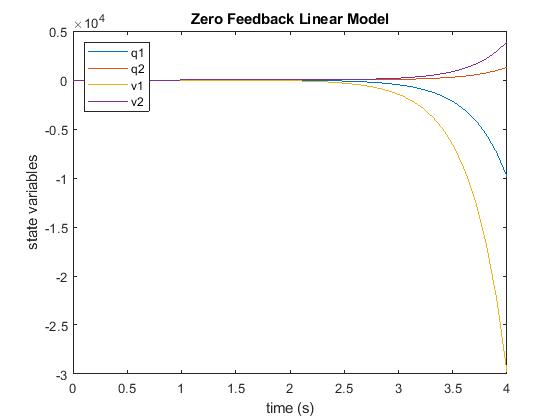
\includegraphics[width=0.8\linewidth]{Zero feedback linear model.jpg}
	\caption{Zero State Feedback Linear Model}
\end{figure}
The graph shown above shows us the same results as taking the eigenvalues of A. We see how the variables don't converge to zero, but rather diverge away, showing us the unstable system with zero state feedback present. \\

Therefore, to make the open-loop system stable, we must find K, for which 4 negative real eigenvalues were chosen to be placed into the acker function as p in Matlab to allow the system to be stable. 
\begin{equation*}
p = \begin{bmatrix}
-4 & -3 & -2 & 1
\end{bmatrix} 
\qquad K = \begin{bmatrix}
12.4544 & -22.0681 &  3.4262&   -4.9472
    \end{bmatrix}
\end{equation*}
To further allow reference tracking, I had to obtain Kref, which is given below, using matrix A,B,C, and K:
\begin{equation*}
    K_{ref} = 1/(-C{(A-BK)^{-1}}B) = -2.6443
\end{equation*}
Now to check if the system is stable, we see if we obtain all real negative eigenvalues when checking the linear system:
\begin{equation*}
    eig(A-BK) = \begin{bmatrix}
      -4.0\\ -3.0\\-1.0\\ -2.0
    \end{bmatrix}\\
\end{equation*}
Showing us that this value of K does provide a stable loop. I then went on to check the steady state error in reference tracking with and without unit disturbance. We calculated steady state error using the Ode45, where dx in the function was given as:
\begin{equation*}
    dx=(A-B*K)*x+B*K_{ref}*r+B*d
\end{equation*}
Where r is the reference point, and d is the disturbance. Thus we set r = 1 and d as 0 or 1 depending on 0 disturbance or unit disturbance. This gave me $y_{ss}$, from which we subtracted r to obtain the steady state error shown below:
\begin{equation*}
    e_{ss0} = 0 \qquad e_{ss1} = -0.37827\\
\end{equation*}

The graphs below shows what the state variables look like over time under steady state error, with and without disturbance. We see how all the variables converge to equilibrium, 0, without disturbance, however when we implement disturbance rejection, it causes $q_{2}$ to converge to its steady state error value of -0.37827.

\begin{figure}[H]
\centering
\begin{minipage}{.5\textwidth}
	\centering
	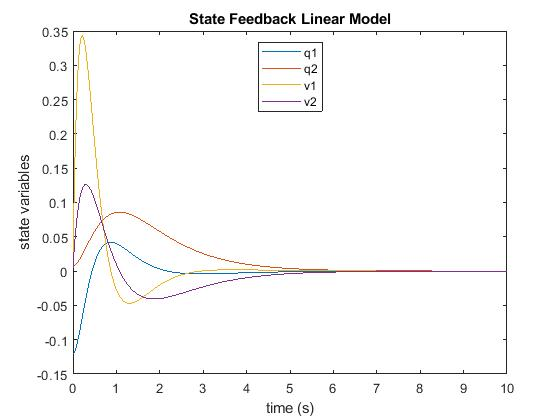
\includegraphics[width=.8\linewidth]{State feedback Linear Model.jpg}
	\caption{linear Model}
	\end{minipage}%
\begin{minipage}{.5\textwidth}
	\centering
	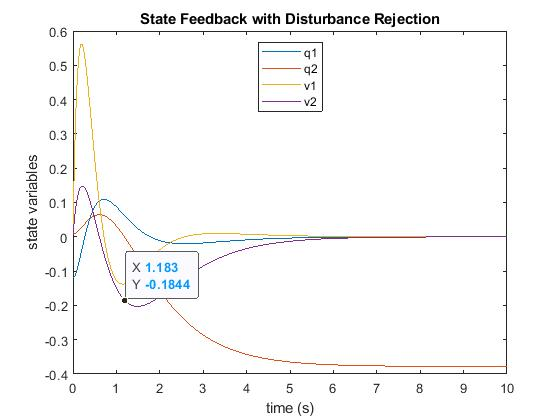
\includegraphics[width=.8\linewidth]{Disturbance rejection.jpg}
	\caption{Disturbance Rejection}
\end{minipage}
\end{figure}

\section{Control Design}
In order for my $q_{2}$ to stabilize at 0, I had to include an input so that:
\begin{equation*}
    \dot{x} = Ax + Bu\\
\end{equation*}
 where,
 \begin{equation*}
    u = -Kx \\
\end{equation*}
and with reference tracking and disturbance rejection,
 \begin{equation*}
    u = -Kx + K_{ref}r + K_{int}v(t)\\
\end{equation*}
Where $K_{int}$ is any number that we decide to pick, and v(t) is an integral, in our case, we set v(t) as 'data.V = sensors.q2-data.r) to allow our actuator to re-adjust itself depending on the reference value, r. I specified $K_{int}$ as 4, an arbitrary value, and r, the reference value as 0.3, a $q_{2}$ value that I desired. We then go on to specify what we want our input as, which is $\tau_{1}$, given as actuator.tau1 in the controller code. This is the only motor that we can control, thus this will be our input $u$ with reference tracking and disturbance rejection as shown above.

\section{Results}

To implement our controller, the MATLAB function:\\ DesignProblem02 ('Controller','datafile','data.mat','tstop',30,'intial',[.8,.8,.3,.3]) will be used to simulate the system. The data that was generated from this function was then imported into a MATLAB program for further analyses to verify whether or not our requirements were true. 
This was done by loading the data through \textbf{load('data.mat'}, followed by defining our variables $(t,q_{1},q_{2},v_{1},v_{2})$ from the processdata, e.g. $q_{2} = processdata.q_{2}$. The error occurring at each time-step was then found between $q_{2}$ and the reference point by $error = abs(r-q_{2})$. If the absolute value of error at the end is reported to be less than or equal to 0.03 radians, within 30 seconds of the controller running, we can verify  that my requirement was met. Therefore,  after running the controller, we get:

\begin{figure}[H]
	\centering
	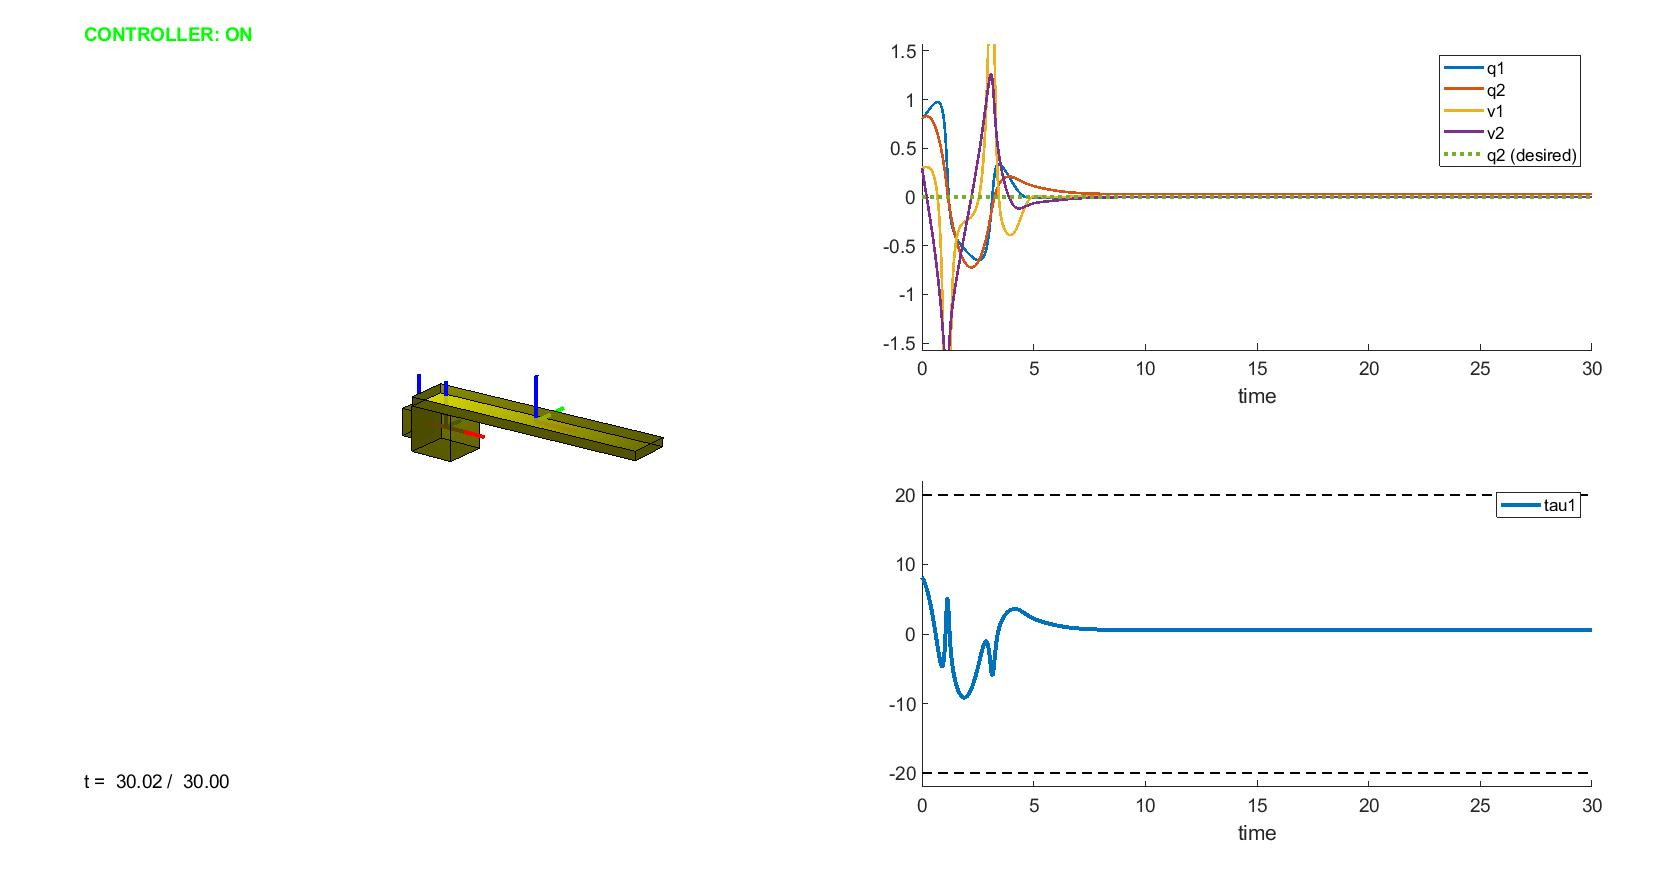
\includegraphics[width=0.8\linewidth]{Controller with disturbance rejection.jpg}
	\caption{Controller Output}
\end{figure}

We can see how overtime, my controller; robot arm, stabilizes, and reaches my desired equilibrium values. We see $q_{2}$ being a little above the desired $q_{2}$ value, however, when we analyze the processed data from data.mat, we see that it is within 0.03 radians of the desired $q_{2}$ value, where it stabilizes at 0.03, exactly within our limits. This shows us how our controller verifies our requirements in this case. We can also see how the arm goes to different reference points before it stabilizes, showing us how it reaches its different values before achieving the desired equilibrium. We see $q_{2}$ go from positive to negative to positive again to negative until it plateau's out at the desired equilibrium value, showing us how it tracks different points before attempting to stabilize. \\

Then analyzing the data that I extracted from data.mat, I plotted state $q_{2}$ w.r.t. time as well as the error of $q_{2}$ w.r.t. time as shown below:

\begin{figure}[H]
\centering
\begin{minipage}{.4\textwidth}
	\centering
	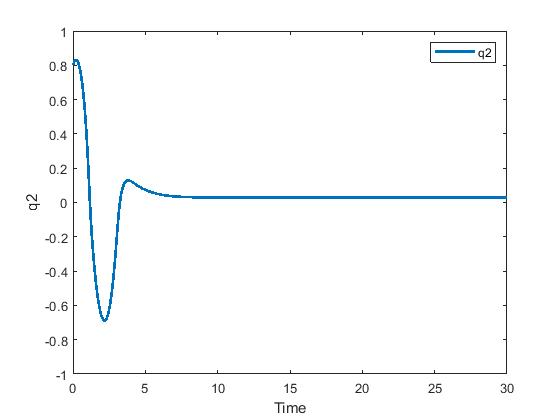
\includegraphics[width=.97\linewidth]{q2 vs time.jpg}
	\caption{$q_{2}$ vs. time}
	\end{minipage}%
\begin{minipage}{.4\textwidth}
	\centering
	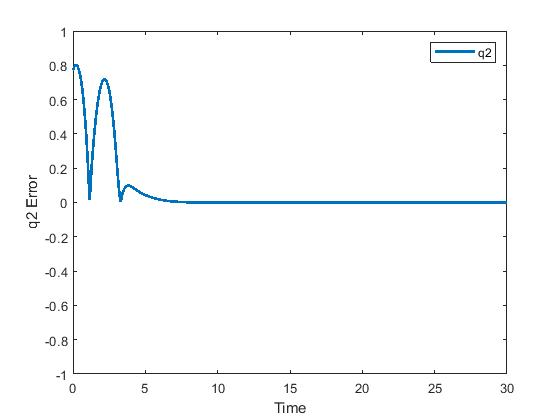
\includegraphics[width=.97\linewidth]{q2 error.jpg}
	\caption{$q_{2,error}$ vs. time}
\end{minipage}
\end{figure}
These graphs show how I reach equilibrium values, and how the error reduces over time to stabilize. We see how initially $q_{2}$ goes a little hay wire, but it starts to stabilize, and remains constant. We can also see how the error for $q_{2}$ overtime reduces, and as it stabilizes, the error becomes 0, showing how the robot arm has reached stability, whilst verifying the requirements that I set.\\ 

If I were to implement the same linearized model in a piece-wise function, we would able to see that my controller reaches stability over time. This would be done by implementing a piece-wise function with regards to an \textit{if, else} statement. An example of that controller is shown below:

\begin{figure}[H]
	\centering
	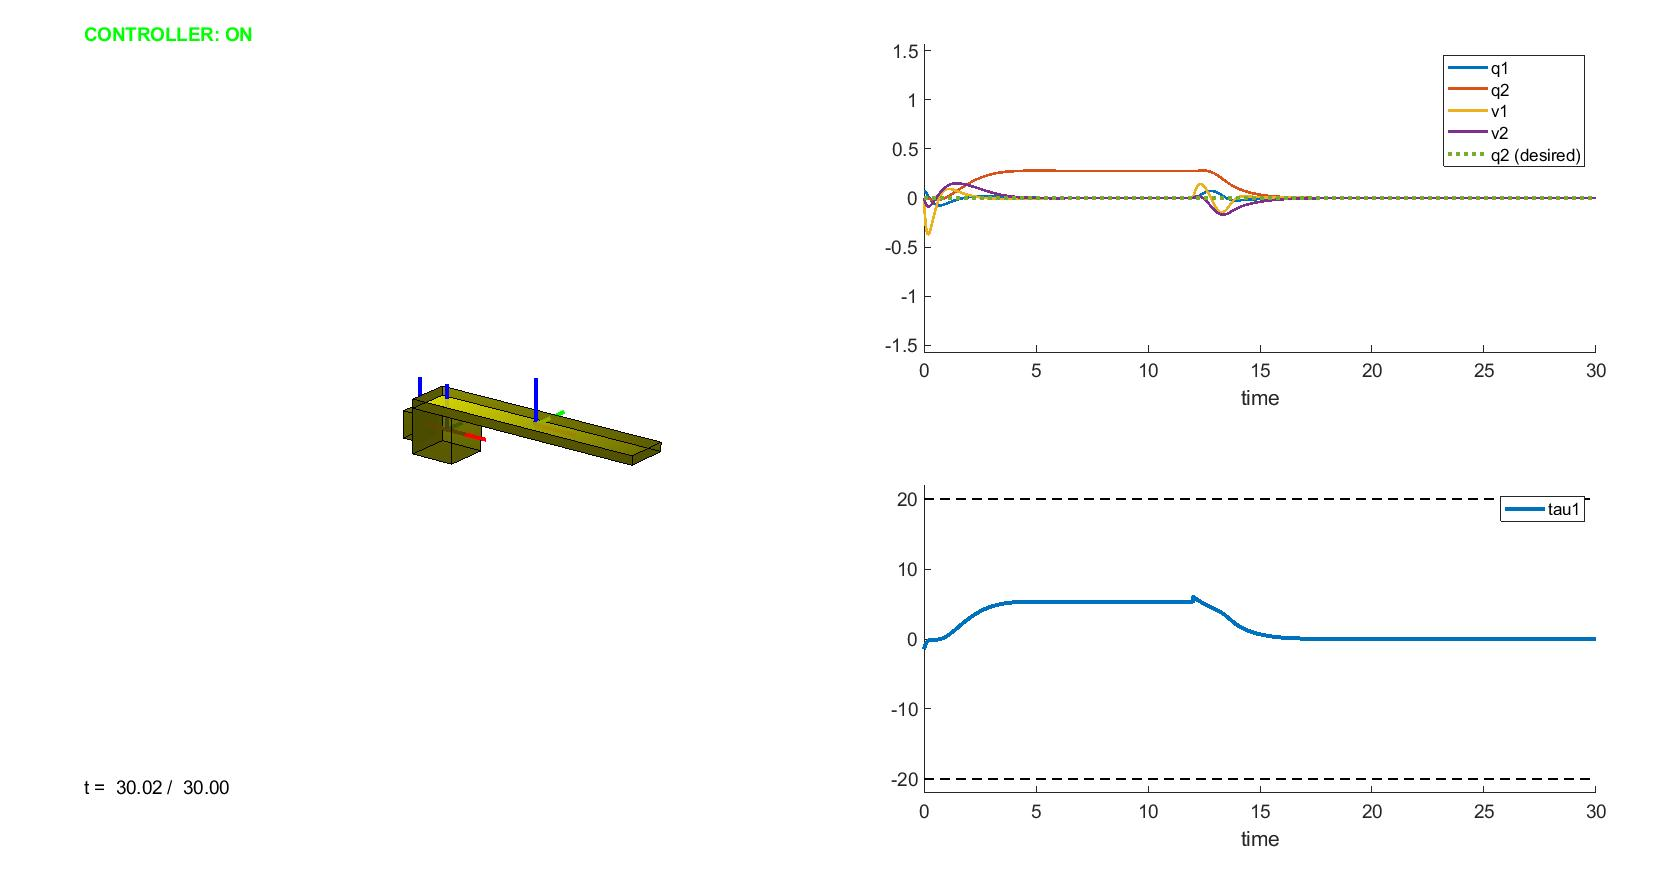
\includegraphics[width=0.7\linewidth]{piece-wise.jpg}
	\caption{Piece-wise Controller Output}
\end{figure}

As shown above, we can see how the system stabilizes within my time requirement, and within the $q_{2}$ error requirement that I defined. Showing us how this system can work under other certain conditions as well. However, if I were to change the initial conditions to something much larger, we would see that the system would not have enough time to stabilize within my defined requirements due to the lack of motor torque as well as the ability to stabilize itself under such conditions. All of this points towards the restrictions that are present with the current system that I have designed, showing us possible places to work on for improvement if it were to be included in future requirements.\\

However, in terms of non-linear controllability, we wouldn't be able to attempt implementing our model through a sinusoidal system of reference points. If we did, we would see that the system would never stabilize as our linear model does not take into account varying fluctuations. The controller would not be able to handle the constantly varying \textit{$q_{1},q_{2},v_{1},v_{2}$}, and would have $q_{2}$ translated by a certain angle from the  desired values. Therefore, there are only certain conditions that allow me to implement our system and successfully run within my defined requirements. This shows us the limitations to the controller that I have designed, and the possible scopes of improvement.
\end{document}
